\documentclass{article}
\usepackage{amssymb}
\usepackage{amsmath}
\usepackage{amsthm}
\usepackage{enumitem}
\usepackage{multicol}

\usepackage{tikz}
\usetikzlibrary{shapes.geometric, arrows}
\tikzstyle{startstop} = [rectangle, rounded corners, minimum width=3cm, minimum height=1cm,text centered, draw=black, fill=white!30]
\tikzstyle{arrow} = [thick,->,>=stealth]

\title{Hw01}
\author{Sean Hinchee and Ryan Radomski}

\begin{document}
\pagenumbering{gobble}

% title part
\title{
Homework \# 1 \\}
\date{September 28, 2017}
\maketitle

% 1
\textbf{1.}
\begin{quote}
$\Pi r.A (\sigma r.B = s.B \land r.A > 55 \land s.H = 100(r \times s))$

\end{quote}

% 2
\textbf{2.}
\begin{quote}
$\Pi r.A (r.A > 55 \land s.H = 100(r \bowtie s))$

\end{quote}

% 3
\textbf{3.}
\begin{quote}
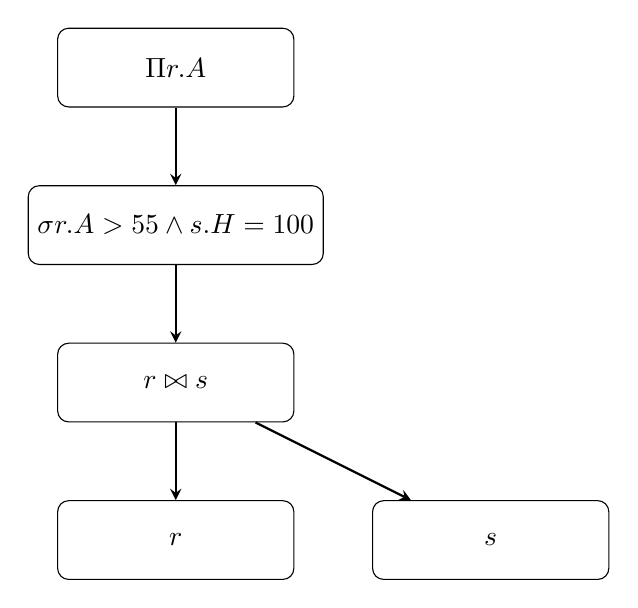
\begin{tikzpicture}[node distance=2cm]
\node (0) [startstop] {$\Pi r.A$};

\node (1) [startstop, below of=0] {$\sigma r.A > 55 \land s.H = 100$ };

\node (2) [startstop, below of=1] {$r \bowtie s$ };

\node (3a) [startstop, below of=2] {$r$ };

\node (3b) [startstop, right of=3a, xshift=2cm] {$s$ };

\draw [arrow] (0) -- (1);

\draw [arrow] (1) -- (2);

\draw [arrow] (2) -- (3a);

\draw [arrow] (2) -- (3b);

\end{tikzpicture}
\end{quote}

% 4
\textbf{4.}
\begin{quote}
% slides p. 64

$r \bowtie s = 800$ pages

$r = 800 * 0.2 = 160$ pages

$s = 1500 * 0.02 = 30$ pages

$ 160 + (30 * \frac{160}{8}) + 800 = $ page accesses $= 1,560$ page accesses

% Gadia book p. 68
Two buffers used, one in, one out.

\end{quote}

% 5
\textbf{5.}
\begin{quote}
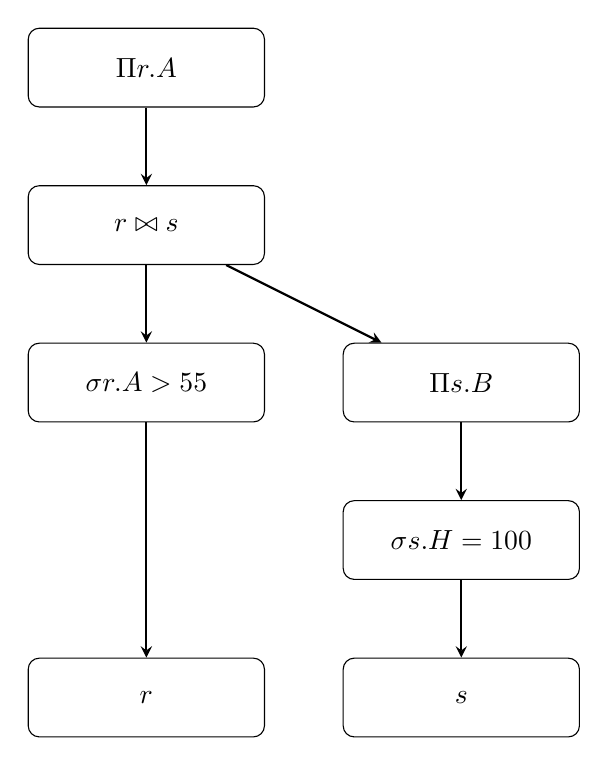
\begin{tikzpicture}[node distance=2cm]
\node (0) [startstop] {$\Pi r.A$};

\node (1) [startstop, below of=0] {$r \bowtie s$ };

\node (2a) [startstop, below of=1] {$\sigma r.A > 55$ };

\node (2b) [startstop, right of=2a, xshift=2cm] {$\Pi s.B$ };

\node (3) [startstop, below of=2b] {$\sigma s.H = 100$ };

\node (4a) [startstop, below of=2a, yshift=-2cm] {$r$ };

\node (4b) [startstop, right of=4a, xshift=2cm] {$s$ };


\draw [arrow] (0) -- (1);

\draw [arrow] (1) -- (2a);

\draw [arrow] (1) -- (2b);

\draw [arrow] (2a) -- (4a);

\draw [arrow] (2b) -- (3);

\draw [arrow] (3) -- (4b);

\end{tikzpicture}

\end{quote}

% 6
\textbf{6.}
\begin{quote}

Preprocess s: $1500 * 0.02 = 30$ pages

2 buffers

Cost of input: $2$ buffers * $800 = 1600$ pages of $r$

Cost for output: $1600 * 0.02 * \frac{10}{10*8} =  4$  page accesses

% not given a size of query output? don't add +3 (s. 73)
Cost of join: $30 + 800 * \frac{4}{8} = 430$ page accesses

10 buffers

Total cost: $(1600 + 4) + 430 = 2034$ page accesses

Buffers: 2 and 10

\end{quote}

% TODO -- maybe
% 7
\textbf{7.}
\begin{quote}

Preprocess r $= 800 * 0.2 = 160$ page accesses

2 buffers

Preprocess s $= 1500 * 0.04 = 60$ page accesses

2 buffers

Cost of input: $4$ buffers * $800 * 1500 = 4,800,000$ pages of $r$ and $s$

Cost for output: $4,800,000 * 0.04 * 0.2 * \frac{10}{10*8} =  4800$  page accesses

% not given a size of query output? don't add +3 (s. 73)
Cost of join: $160 + 60 + 800 * \frac{4800}{8} = 480,220$ page accesses

10 buffers

Total cost: $(4,800,000 + 4800) + 480,220 = 5,285,020$ page accesses

Buffers: 4 and 10

\end{quote}

% 8
\textbf{8.}
\begin{quote}

% s. 70
$m = 3$

Input r: 800 pages accesses

Input s: $30000 * 3$ page accesses

Output: $1500 * 0.02$ page accesses

Total: $800 + 30000 * 3 * 0.02 + 1500 * 0.02 = 2,630$

\end{quote}

% 9
\textbf{9.}
\begin{quote}

Preprocess r: 

Cost $= 800 + (800 * 0.2) = 960$ page accesses

reduced size = 160 pages

2 buffers

Preprocess s:

Cost $= 1500+10=1510$ page accesses

2 buffers

Sort reduced r:

$2 * 160 * log_{10}(160) = 2 * 160 * 2 = 640$ page accesses

10 buffers

Sort reduced s:

$2 * 1510 * log_{10}(1510) = 2 * 1510 * 3 = 9000$ page accesses

10 buffers

Join by merging:

$160+10+3=173$ pages accesses

Total cost: $960+1510+640+9000+173+3=12286$

3 buffers

Buffers: 2, 10, and 3

\end{quote}

\end{document}
